\indent\indent You can perform separate grid calculation on a single analysis. To do so, draw several grids before starting a correlation in the grid creation tool. Once the calculation done, you'll be able to analyze these grid separately.\\
\newline
\indent If several grids have been created, they'll be dissociated in the visualisation tool. You are then able to differentiate the strain in one grid compared to another. Using the instance management tool, you can temporaly hide one or several grids to focus on the one (or those) that you're interested in.
\begin{itemize}
  \item Go into \textit{Masks \textgreater Manage Grids}
  \item Chose the grids you want to hide/display
  \item Validate to apply changes
\end{itemize}
\newline

\begin{figure}[!h]
   \centering
   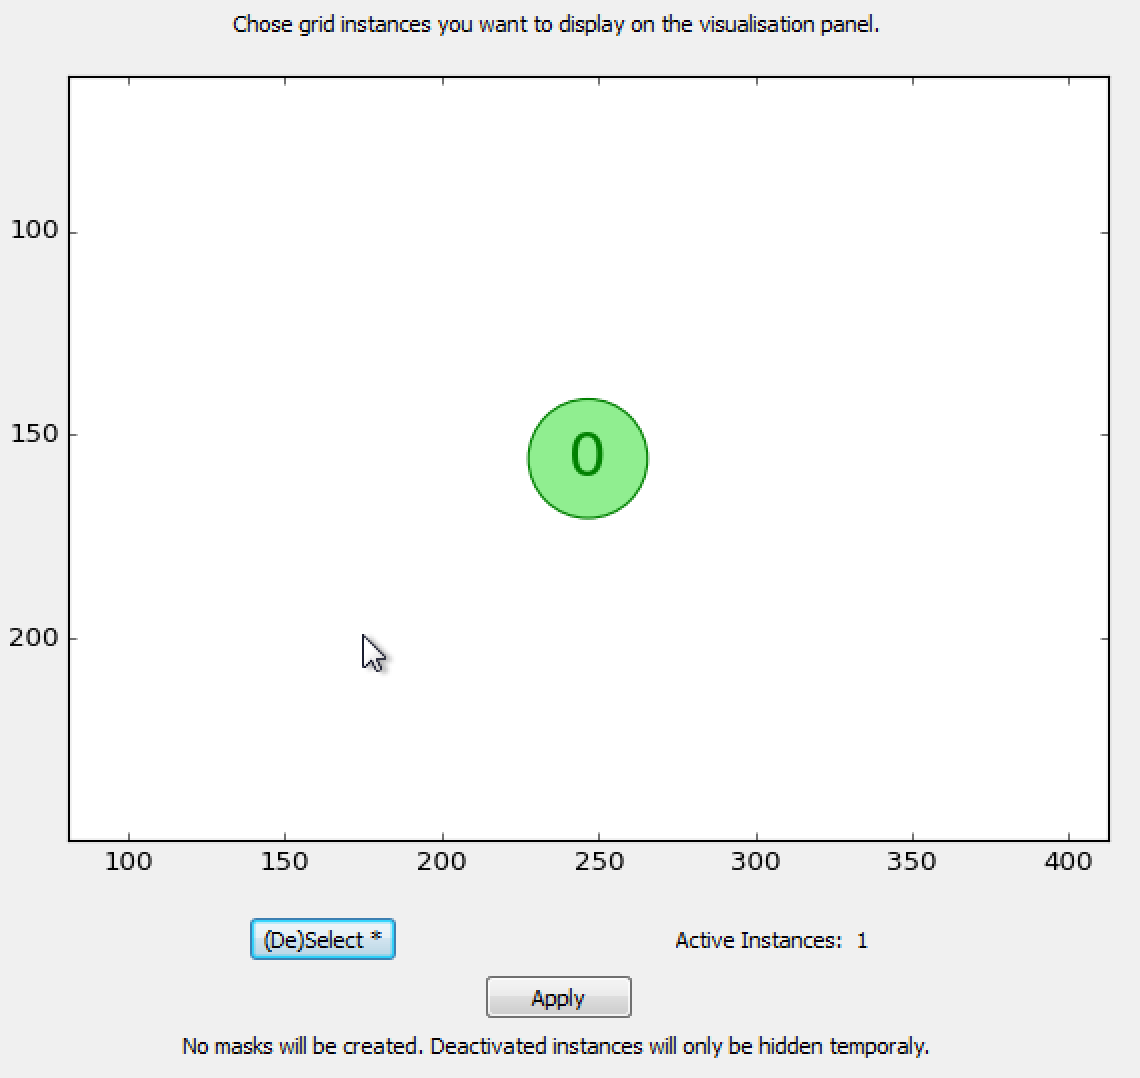
\includegraphics[scale=.4]{grid_management}
   \caption{Grid Management - Active instances displayed in green}
\end{figure}

When you hide or display grid instances, the changes made are not saved and all the grid will be displayed by default on the next start-up.
